
\section{Second Article Section}
    \paragraph{}
    sed quia non numquam eius modi tempora incidunt ut labore et dolore magnam aliquam quaerat voluptatem. Ut enim ad minima
    veniam, quis nostrum exercitationem ullam corporis suscipit laboriosam, nisi ut aliquid ex ea commodi

    \begin{figure}[h!]
        \centering
        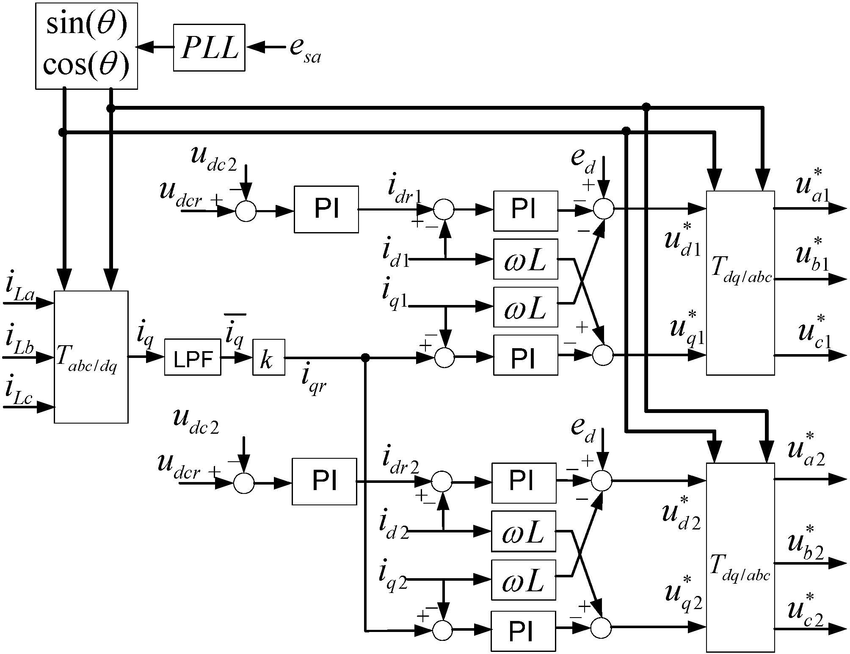
\includegraphics[scale=0.3]{assets/figures/figure_1.png}
        \caption{This is the caption of the first figure}
        \label{fig:figure of something}
    \end{figure}
    
    \subsection{This is a subsection}
    \paragraph{}
    Lorem ipsum dolor sit amet, consectetur adipiscing elit, sed do eiusmod tempor incididunt ut labore et dolore magna aliqua.
    Ut enim ad minim veniam, quis nostrud exercitation ullamco laboris nisi ut aliquip ex ea commodo consequat. Duis aute irure
    dolor in reprehenderit in voluptate velit esse cillum dolore eu fugiat nulla pariatur. See Figure \ref{fig:figure of something}
    Excepteur sint occaecat cupidatat non proident, sunt in culpa qui officia deserunt mollit anim id est laborum.

    \subsection{This is a subsection}
    \paragraph{}
    Sed ut perspiciatis unde omnis iste natus error sit voluptatem accusantium doloremque laudantium, totam rem aperiam,
    eaque ipsa quae ab illo inventore veritatis et quasi architecto beatae vitae dicta sunt explicabo. Nemo enim ipsam
    voluptatem quia voluptas sit aspernatur aut odit aut fugit, sed quia consequuntur magni dolores eos qui ratione
    voluptatem sequi nesciunt. Neque porro quisquam est, qui dolorem ipsum quia dolor sit amet, consectetur, adipisci
    velit, consequatur? Quis autem vel eum iure reprehenderit qui in ea voluptate velit esse quam nihil molestiae
    consequatur, vel illum qui dolorem eum fugiat quo voluptas nulla pariatur?

    \begin{table}[h!]
        \centering
        \caption{Fisher's Iris data}
        \label{tab:table1}
        % This is to resize the table to fit the page
        \resizebox{\linewidth}{!}{%
        % With l,c,r you define the alignment of each column
        \begin{tabular}{l||c|c|c|c|r}
            Dataset Order & Sepal Length & Sepal Width & Petal Length & Petal Length & Species\\
            \hline
            1 &	5.1 & 3.5 & 1.4 & 0.2 & I. setosa\\
            2 &	4.9 & 3.0 & 1.4 & 0.2 & I. setosa\\
            3 &	4.7 & 3.2 & 1.3 & 0.2 & I. setosa\\
            4 &	4.6 & 3.1 & 1.5 & 0.2 & I. setosa\\
        \end{tabular}
        }
    \end{table}

% It creates a nice aesthetic to start a new chapter/section in a new page
\newpage
